% This LaTeX was auto-generated from MATLAB code.
% To make changes, update the MATLAB code and export to LaTeX again.

\documentclass{article}

\usepackage[utf8]{inputenc}
\usepackage[T1]{fontenc}
\usepackage{lmodern}
\usepackage{graphicx}
\usepackage{color}
\usepackage{hyperref}
\usepackage{amsmath}
\usepackage{amsfonts}
\usepackage{epstopdf}
\usepackage[table]{xcolor}
\usepackage{matlab}

\sloppy
\epstopdfsetup{outdir=./}
\graphicspath{ {./Lab06_images/} }

\begin{document}

\matlabtitle{LAB 6: DESIGN OF SPEED ESTIMATOR for DC MOTOR}

\begin{matlabcode}
%---------------------------------------
% Fill in your student Name and ID.
Students.Name = 'Seyed Yazdan Zinati';
Students.ID = '260928077';
%---------------------------------------
\end{matlabcode}


\matlabheading{\textbf{0. Objectives}}

\begin{par}
\begin{flushleft}
In this lab, we will use the angular velocity measurements from the DC Motor to estimate the full state of the DC Motor, i.e. angular velocity and the current. We will use \texttt{\textbf{MATLAB}} to place the poles of the Luenberger observer and run a state estimator both in continuous and discrete time.
\end{flushleft}
\end{par}

\begin{par}
\begin{flushleft}
To initiate a connection with the virtual motor, run the following:
\end{flushleft}
\end{par}

\begin{matlabcode}
Motor = VirtualMotor();
\end{matlabcode}


\matlabheading{\textbf{1. A State-Space Representation of DC Motor}}

\begin{par}
\begin{flushleft}
A DC motor is a device that converts armature current into mechanical torque. A schematic of a DC motor is shown in the following
\end{flushleft}
\end{par}

\begin{par}
\begin{flushleft}
\textless{}\textless{}fig\_dcmotorshematic.png\textgreater{}\textgreater{}
\end{flushleft}
\end{par}

\begin{par}
\begin{flushleft}
We can model the DC motor using the armature current $i$ and the angular speed $\omega$. The dynamics of the DC motor are given by the following two coupled differential equations:
\end{flushleft}
\end{par}

\begin{par}
$$J{{\frac{d\omega }{dt}+b\omega =K_t i}}$$
\end{par}

\begin{par}
$$L{{\frac{di}{dt}+Ri=v-K_e \omega }}$$
\end{par}

\begin{par}
\begin{flushleft}
where the parameters are defined as follow
\end{flushleft}
\end{par}

\begin{matlabcode}
Param.Kt = 0.034; % Torque proportionality constant (Kg m2 /s2/A) (N.m/A)
Param.Ke = 0.034; % Back electromotive proportionality constant (V/rad/s)
Param.L = 0.018; % Electric inductance (H)
Param.R = 8.4; % Terminal resistance (Ohm)
Param.J = 2e-05; % Rotor moment of inertia (kg.m2)
Param.b = 1e-05; % Rotor viscous friction constant (Kg.m2/s) (N.m.s)
\end{matlabcode}


\begin{par}
\begin{flushleft}
From these differential equations we can represent the DC Motor model by the following state-space representation
\end{flushleft}
\end{par}

\begin{par}
$${{\frac{d}{dt}x(t)=\left(\begin{array}{cc}
-{{\frac{b}{J}}} & {{\frac{K_t }{J}}}\\
-{{\frac{K_e }{L}}} & -{{\frac{R}{L}}}
\end{array}\right)x(t)+\left(\begin{array}{c}
0\\
{{\frac{1}{L}}}
\end{array}\right)v(t)}}$$
\end{par}

\begin{par}
\begin{flushleft}
where $v(t)$ is the voltage and the state vector contains the angular velocity $\omega (t)$ and the current $i(t)$
\end{flushleft}
\end{par}

\begin{par}
$$x(t)=\left(\begin{array}{c}
\omega (t)\\
i(t)
\end{array}\right)$$
\end{par}

\begin{par}
\begin{flushleft}
Note that if we think of the angular velocity $\omega (t)$ as the output of this system, then $C=\left(\begin{array}{cc}
1 & 0
\end{array}\right)$ and
\end{flushleft}
\end{par}

\begin{par}
$$\omega (t)=Cx(t)$$
\end{par}

\begin{par}
\begin{flushleft}
In this case, the transfer function from the voltage $v(t)$ to the angular velocity $\omega (t)$ is given by
\end{flushleft}
\end{par}

\begin{par}
$$G_o (s)=C(sI-A)^{-1} B$$
\end{par}

\begin{par}
\begin{flushleft}
The state-space representation of the DC Motor can be written as
\end{flushleft}
\end{par}

\begin{matlabcode}
A = [ ...
    -Param.b / Param.J, Param.Kt / Param.J; ...
    -Param.Ke / Param.L, -Param.R / Param.L]
\end{matlabcode}
\begin{matlaboutput}
A = 2x2    
1.0e+03 *

   -0.0005    1.7000
   -0.0019   -0.4667

\end{matlaboutput}
\begin{matlabcode}
B = [ ...
    0; ...
    1 / Param.L];
C = [1, 0]
\end{matlabcode}
\begin{matlaboutput}
C = 1x2    
     1     0

\end{matlaboutput}
\begin{matlabcode}
D = 0;
Go = ss(A, B, C, D);
tf(Go)
\end{matlabcode}
\begin{matlaboutput}
ans =
 
        9.444e04
  --------------------
  s^2 + 467.2 s + 3444
 
Continuous-time transfer function.
\end{matlaboutput}


\matlabheading{\textit{Question 1 (1 mark)}}

\begin{par}
\begin{flushleft}
Using \texttt{\textbf{MATLAB}}, compute the eigenvalues of the observability matrix of the system? Based on the eigenvalues, is the system observable?
\end{flushleft}
\end{par}

\begin{matlabcode}
% Eigenvalues of [C, C A] for Go
Obs = [C; C*A]
\end{matlabcode}
\begin{matlaboutput}
Obs = 2x2    
1.0e+03 *

    0.0010         0
   -0.0005    1.7000

\end{matlaboutput}
\begin{matlabcode}
eigenValues = eig(Obs)
\end{matlabcode}
\begin{matlaboutput}
eigenValues = 2x1    
        1700
           1

\end{matlaboutput}
\begin{matlabcode}

% Is the system observable?
det(Obs)
\end{matlabcode}
\begin{matlaboutput}
ans = 1700
\end{matlaboutput}
\begin{matlabcode}

if det(Obs) ~= 0
    disp('The system is observable')
end
\end{matlabcode}
\begin{matlaboutput}
The system is observable
\end{matlaboutput}


\matlabheading{\textbf{2. State Estimator Design}}

\begin{par}
\begin{flushleft}
Knowing the system state is necessary to solve many control problems; for example, stabilizing a system using state feedback. In most practical cases, the physical state of the system cannot be determined by direct observation. Instead, indirect effects of the internal state are observed by way of the system outputs. A simple example is that of vehicles in a tunnel: the rates and velocities at which vehicles enter and leave the tunnel can be observed directly, but the exact state inside the tunnel can only be estimated. If a system is observable, it is possible to fully reconstruct the system state from its output measurements using the state observer.
\end{flushleft}
\end{par}

\begin{par}
\begin{flushleft}
In this lab, we assume that the full state feedback is not available and only the angular speed ($\omega (t)$) is available. The angular velocity measured directly from the DC Motor is affected by an unwanted noise. The sensor noise can vary greatly as it is produced by several different effects, however, it is usually approximated to an additive white Gaussian noise. In this case, the intensity of the noise can be measured by its variance.
\end{flushleft}
\end{par}

\begin{par}
\begin{flushleft}
The objective of this state estimator will be to:
\end{flushleft}
\end{par}

\begin{enumerate}
\setlength{\itemsep}{-1ex}
   \item{\begin{flushleft} Estimate the current $i(t)$. \end{flushleft}}
   \item{\begin{flushleft} Reduce the variance of the sensor noise in both the angular velocity and the current estimates. \end{flushleft}}
\end{enumerate}

\begin{par}
\begin{flushleft}
In \texttt{\textbf{MATLAB}}, the function \texttt{\textbf{place}} is designed for choosing the controller gain $K$. Yet by using the duality between choosing controller gain $K$ and choosing estimator gain $L$ we can use \texttt{\textbf{place}} to identify the gain $L$.
\end{flushleft}
\end{par}

\matlabheading{\textit{Question 2 (1 mark)}}

\begin{par}
\begin{flushleft}
Using the \texttt{\textbf{place}} command design a state estimator gain $L$ for the system ($A,\,C$) such that the eigenvalues of the estimation error are $P_{1,2} =-50\pm 50j$.
\end{flushleft}
\end{par}

\begin{matlabcode}
p1 = 50 * (-1 + 1j);
p2 = 50 * (-1 - 1j);

% the gain L (use place)

L = place(A', C', [p1,p2])'
\end{matlabcode}
\begin{matlaboutput}
L = 2x1    
 -367.1667
  101.7059

\end{matlaboutput}


\begin{par}
\begin{flushleft}
The dynamics of the Luenberger observer are
\end{flushleft}
\end{par}

\begin{par}
$${{\frac{d}{dt}\hat{x} (t)=A\hat{x} (t)+Bu(t)+L(y(t)-\hat{y} (t))}}$$
\end{par}

\begin{par}
\begin{flushleft}
The error of the Luenberger observer is defined by $e(t)=\hat{x} (t)-x(t)$.
\end{flushleft}
\end{par}

\matlabheading{\textit{Question 3 (1 mark)}}

\begin{par}
\begin{flushleft}
Write the $A$ matrix of the Luenberger error dynamics and complete the code to see how the error converges to zero when starting with wrong initial values.
\end{flushleft}
\end{par}

\begin{matlabcode}
Ae = A - L * C
\end{matlabcode}
\begin{matlaboutput}
Ae = 2x2    
1.0e+03 *

    0.3667    1.7000
   -0.1036   -0.4667

\end{matlaboutput}
\begin{matlabcode}

Be = [0; 0];
Ce = eye(2);
De = 0;
Ge = ss(Ae, Be, Ce, De);

% simulate the error starting from wrong initial values
t = 0:0.01:2;
e = lsim(Ge, zeros(size(t)), t, [100, 1])';

% Answer here retrieve wErr and eErr from e

wErr = e(1, :);
iErr = e(2, :);

figure;
clf;
subplot(2, 1, 1)
hold on
plot(t, wErr);
xlabel('Time (s)')
ylabel('Angular velocity (rad/s)')
title(sprintf('Student ID %s - Luenberger error.', Students.ID));
grid on
subplot(2, 1, 2)
hold on
plot(t, iErr);
xlabel('Time (s)')
ylabel('Current (A)')
grid on
\end{matlabcode}
\begin{center}
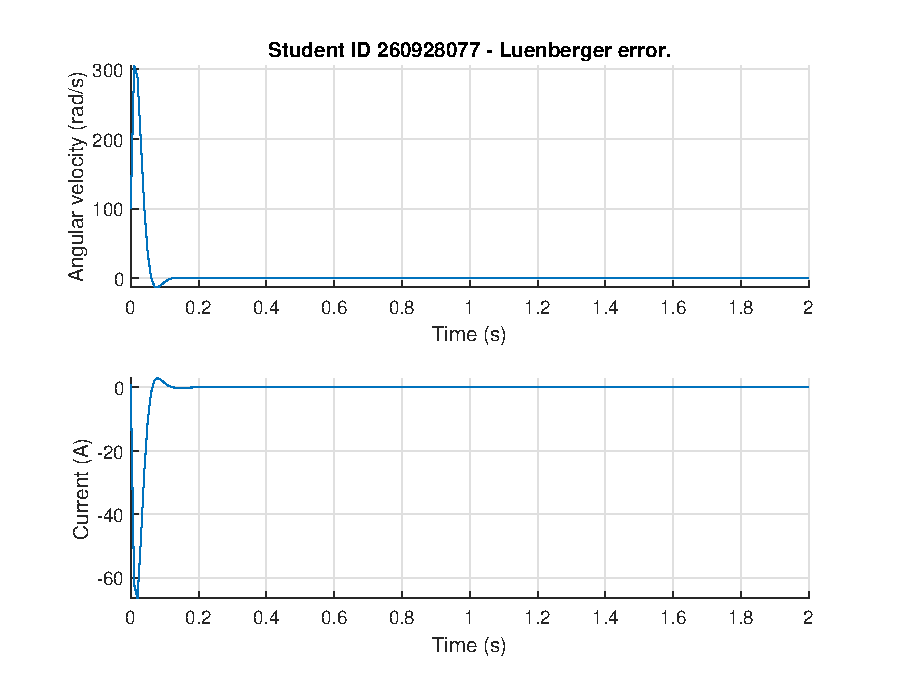
\includegraphics[width=\maxwidth{56.196688409433015em}]{figure_0.eps}
\end{center}


\matlabheading{\textit{3. Open Loop Observer Design}}

\begin{par}
\begin{flushleft}
In this section we want to use the estimator designed above to estimate the states of the DC motor in an open loop structure. The representation of an open loop system with an estimator is given as follows:
\end{flushleft}
\end{par}

\begin{par}
\begin{flushleft}
\textless{}\textless{}fig\_lab06\_estimator.png\textgreater{}\textgreater{}
\end{flushleft}
\end{par}

\begin{par}
\begin{flushleft}
As you see, the estimator is like a parallel system that receives the input and output of the system and generates an estimate of the states.
\end{flushleft}
\end{par}

\begin{par}
\begin{flushleft}
We will generate a set of measurements for angular velocity from the DC Motor. For this we run the following experiment
\end{flushleft}
\end{par}

\begin{matlabcode}
T = 10; % Simulation duration
dt = 0.01; % Simulation step time
t = 0:dt:T; % Time array
TStart = 5; % Step start
wRef = zeros(size(t));
wRef(t < TStart) = 25;
wRef(t >= TStart) = 75;

N = 1 / (C * (-A)^(-1) * B);
Motor.reset();
Motor.input(N*wRef);
Motor.off();

Motor.save(Students, 'Lab06.Data_Collection');


% Get results of driving Virtual DC Motor
v = Motor.voltage(t <= T);
i = Motor.current(t <= T);
w = Motor.velocity(t <= T);

% Plot results
figure;
clf;
subplot(2, 1, 1)
title(sprintf('Student ID %s - A step response experiment', Students.ID));
plot(t, w)
legend('Angular velocity (rad/s)', ...
    'location', 'best');
xlim([TStart - 1, T])
grid on
subplot(2, 1, 2)
plot(t, i)
legend('Current (A)', 'location', 'best');
xlim([TStart - 1, T])
grid on
\end{matlabcode}
\begin{center}
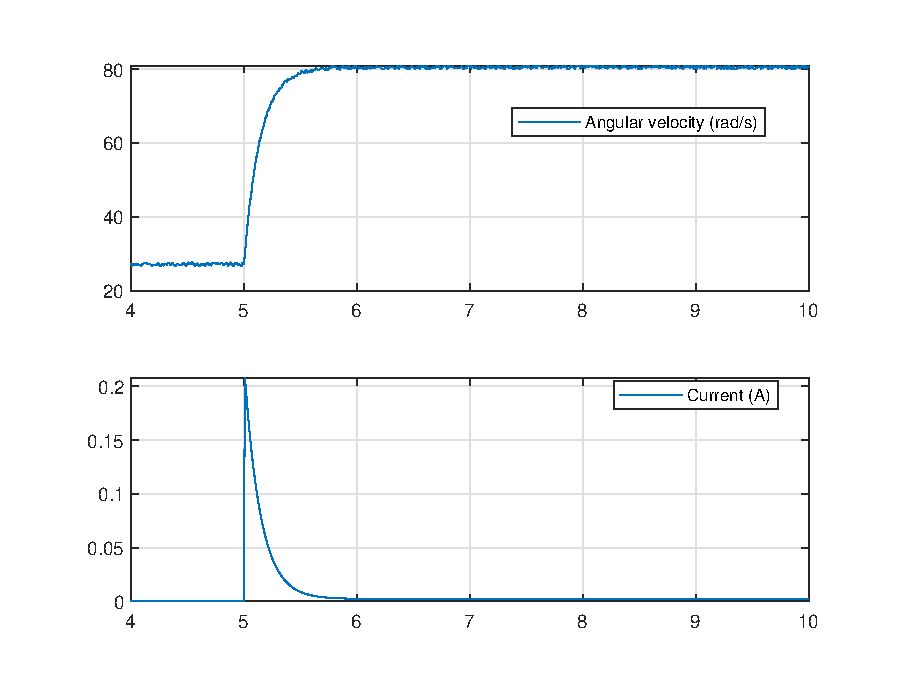
\includegraphics[width=\maxwidth{56.196688409433015em}]{figure_1.eps}
\end{center}


\begin{par}
\begin{flushleft}
Since we are manipulating the DC Motor in discrete time, we cannot use gains designed for the continuous system. We will need to convert these gains to their equivalent discrete gains.
\end{flushleft}
\end{par}

\begin{par}
\begin{flushleft}
First we define the system $G_o$ in a discrete form using the \texttt{\textbf{c2d}} function
\end{flushleft}
\end{par}

\begin{matlabcode}
Go_d = c2d(Go, dt, 'zoh')
\end{matlabcode}
\begin{matlaboutput}
Go_d =
 
  A = 
              x1         x2
   x1      0.942       3.45
   x2  -0.003834  -0.004108
 
  B = 
           u1
   x1   1.563
   x2  0.1132
 
  C = 
       x1  x2
   y1   1   0
 
  D = 
       u1
   y1   0
 
Sample time: 0.01 seconds
Discrete-time state-space model.
\end{matlaboutput}


\begin{par}
\begin{flushleft}
Now if $L$ is a Luenberger gain for ($A$, $C$) which places poles ($p_1$, $p_2$) . The equivalent $L_d$ gain will place the discrete poles ($\exp (p_1 T_s )$, $\exp (p_2 T_s )$) for the discrete system ($A_d$, $C_d$) . As an example, we can write
\end{flushleft}
\end{par}

\begin{matlabcode}
Ad = Go_d.A;
Bd = Go_d.B;
Cd = Go_d.C;
Ld = place(Ad', Cd', exp([p1, p2]*dt))'
\end{matlabcode}
\begin{matlaboutput}
Ld = 2x1    
   -0.1267
    0.1041

\end{matlaboutput}


\begin{par}
\begin{flushleft}
Finally, we should write the Luenberger equation in a discrete time:
\end{flushleft}
\end{par}

\begin{par}
$$\hat{x} (n+1)=A_d \hat{x} (n)+B_d u(n)+L_d (y(n)-\hat{y} (n))$$
\end{par}

\begin{par}
\begin{flushleft}
where ($A_d$, $B_d$) are discrete form of ($A$, $B$), and $L_d$ is the equivalent Luenberger gain of $L$ in discrete time.
\end{flushleft}
\end{par}

\matlabheading{\textit{Question 4 (2 marks)}}

\begin{par}
\begin{flushleft}
For the desired poles $P_{1,2} =-50\pm 50j$ of the Luenberger observer, complete the following code to design and test the state estimator.
\end{flushleft}
\end{par}

\begin{matlabcode}
p1 = 50 * (-1 + 1j);
p2 = 50 * (-1 - 1j);

% Find the gain Ld

Ld = place(Ad', Cd', exp([p1, p2] * dt))'
\end{matlabcode}
\begin{matlaboutput}
Ld = 2x1    
   -0.1267
    0.1041

\end{matlaboutput}
\begin{matlabcode}

% Simulate state estimation
xHat = zeros(2, length(t));
for n = 1:length(t) - 1
    v_ = N * wRef(n);
    % Write the estimator dynamics here
    
    xHat(:, n+1) = Ad*xHat (:, n)+Bd* v_+Ld*(w(n)-Cd*xHat (:, n));
    
end
\end{matlabcode}


\begin{matlabcode}
% Plot results
figure;
clf;

subplot(2, 1, 1)
title(sprintf('Student ID %s - State Estimator Test', Students.ID));
% Superpose the actual angular velocity and the estimated angular velocity
plot(t, w)
hold on
plot(t, xHat(1, :))

legend('Angular velocity (rad/s)', ...
    'Estimated angular velocity (rad/s)', ...
    'location', 'best');
xlim([TStart - 1, T])
grid on
subplot(2, 1, 2)

% Plot current
plot(t, i)
hold on
plot(t, xHat(2, :))

legend('Current (A)', 'Estimated Current (A)', 'location', 'best');
xlim([TStart - 1, T])
grid on
\end{matlabcode}
\begin{center}
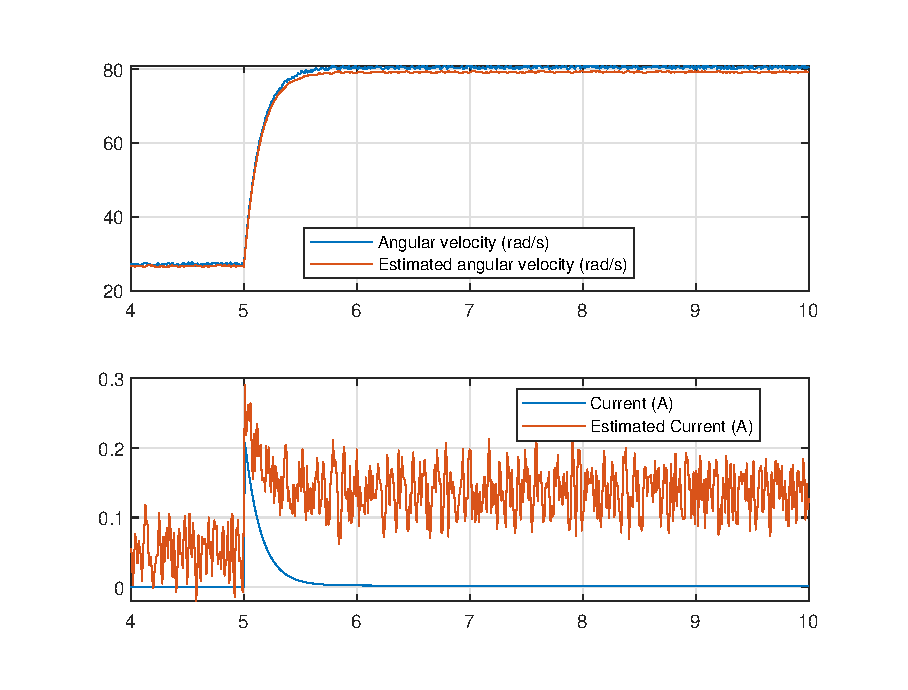
\includegraphics[width=\maxwidth{56.196688409433015em}]{figure_2.eps}
\end{center}


\matlabheading{\textit{Question 5 (1 marks)}}

\begin{par}
\begin{flushleft}
1. A discrete observer is called asymptotically stable if the observer error $e(n)=x(n)-\hat{x} (n)$ converges to zero when $n\to \infty$. For a discrete Luenberger observer, the observer error satisfies $e(n+1)=(A_d -L_d C_d )e(n)$ and therefore the Luenberger observer for this discrete-time system is asymptotically stable if and only if all of the eigenvalues of $(A_d -L_d C_d )$ are all inside the unit circle. Compute the eigenvalues of $(A_d -L_d C_d )$ in discrete time and determine whether the observer is asymptotically stable or not.
\end{flushleft}
\end{par}

\begin{matlabcode}
eigenValues = eig(Ad - Ld * Cd)
\end{matlabcode}
\begin{matlaboutput}
eigenValues = 2x1 complex    
   0.5323 + 0.2908i
   0.5323 - 0.2908i

\end{matlaboutput}
\begin{matlabcode}
% All eigenvalues are inside the unit circle, the observer is 
% asymptotically stable 
\end{matlabcode}


\begin{par}
\begin{flushleft}
2. Based on the plot of the error in question 4, does the error go to zero? Does this confirm the asymptotically stability of the observer? If not justify your answer.
\end{flushleft}
\end{par}

\begin{matlabcode}
% The difference between the actual value and the estimated value
% does not converge to 0. Even though the value is close to zero, 
% it is marginally large compared to the reference current. 
% So we can conclude that the Observer is not asymptotically stable yet. 
\end{matlabcode}


\begin{par}
\begin{flushleft}
We can evaluate the goodness of the estimate by measuring the noise transmitted to the observer.
\end{flushleft}
\end{par}

\begin{matlabcode}
error_w = std(xHat(1, t > 6));
error_i = std(xHat(2, t > 6));
fprintf('Student ID %s - using gain [%.3f;%.3f]: error in angular velocity: %.3f - error in current: %.3f.\n', ...
    Students.ID, Ld, error_w, error_i);
\end{matlabcode}
\begin{matlaboutput}
Student ID 260928077 - using gain [-0.127;0.104]: error in angular velocity: 0.134 - error in current: 0.033.
\end{matlaboutput}


\matlabheading{\textit{Question 6 (3.0 marks)}}

\begin{par}
\begin{flushleft}
Repeat question 4 for the following other poles
\end{flushleft}
\end{par}

\begin{enumerate}
\setlength{\itemsep}{-1ex}
   \item{\begin{flushleft} $\displaystyle P_{1,2} =-250\pm 250j$ \end{flushleft}}
   \item{\begin{flushleft} $\displaystyle P_{1,2} =-500\pm 500j$ \end{flushleft}}
\end{enumerate}

\begin{par}
\begin{flushleft}
Based on the standard deviation of the observed noise, which poles you choose for the observer?
\end{flushleft}
\end{par}

\begin{matlabcode}
p1 = 250 * (-1 + 1j);
p2 = 250 * (-1 - 1j);

% Rerun the state estimator and calculate errors

Ld = place(Ad', Cd', exp([p1, p2] *dt))';

% Simulate state estimation
xHat = zeros(2, length(t));
for n = 1:length(t) - 1
    v_ = N * wRef(n);
    xHat(:, n+1) = Ad*xHat (:, n)+Bd*v_+Ld*(w(n)-Cd*xHat (:, n));
end
error_w = std(xHat(1, t>6));
error_i = std(xHat(2, t>6));

fprintf('Student ID %s - using gain [%.3f;%.3f]: error in angular velocity: %.3f - error in current: %.3f.\n', ...
    Students.ID, Ld, error_w, error_i);
\end{matlabcode}
\begin{matlaboutput}
Student ID 260928077 - using gain [1.069;-0.002]: error in angular velocity: 0.311 - error in current: 0.001.
\end{matlaboutput}


\begin{matlabcode}
p1 = 500 * (-1 + 1j);
p2 = 500 * (-1 - 1j);

% Rerun the state estimator and calculate errors

Ld = place(Ad', Cd', exp([p1, p2]*dt))';

% Simulate state estimation
xHat = zeros(2, length(t));
for n = 1:length(t) - 1
    v_ = N * wRef(n);
    xHat(:, n+1) = Ad*xHat (:, n)+Bd*v_+Ld*(w(n)-Cd*xHat (:,n));
end
error_w = std(xHat(1, t>6));
error_i = std(xHat(2, t>6));

fprintf('Student ID %s - using gain [%.3f;%.3f]: error in angular velocity: %.3f - error in current: %.3f.\n', ...
    Students.ID, Ld, error_w, error_i);
\end{matlabcode}
\begin{matlaboutput}
Student ID 260928077 - using gain [0.934;-0.004]: error in angular velocity: 0.269 - error in current: 0.001.
\end{matlaboutput}


\begin{matlabcode}
% which poles you choose for the observer?
% I choose the poles that give us the lowest errors
% poles with lowest errors are : 
% p1 = 500 * (-1 + 1j);
% p2 = 500 * (-1 - 1j);
\end{matlabcode}


\matlabheading{\textbf{3. Closed-loop State Estimator for Velocity Control}}

\begin{par}
\begin{flushleft}
In this section, we want to use the estimated states with a state feedback controller to track a reference input, while satisfying the three specifications.
\end{flushleft}
\end{par}

\begin{itemize}
\setlength{\itemsep}{-1ex}
   \item{\begin{flushleft} Overshoot less than 20\%. \end{flushleft}}
   \item{\begin{flushleft} 5\%-settling time less than 0.25 seconds. \end{flushleft}}
   \item{\begin{flushleft} Steady state gain of 1 $\pm$ 5\%. \end{flushleft}}
\end{itemize}

\begin{par}
\begin{flushleft}
The state feedback input to the system is
\end{flushleft}
\end{par}

\begin{par}
$$v(t)=N\omega_{ref} (t)-Kx(t)$$
\end{par}

\begin{par}
\begin{flushleft}
Because the observation of the system is not complete and we don't have access to the full state of the system, we use the following control law instead:
\end{flushleft}
\end{par}

\begin{par}
$$v(t)=N\omega_{ref} (t)-K\hat{x} (t)$$
\end{par}

\begin{par}
\begin{flushleft}
where $K$ and $N$ are computed to satisfy the specifications.
\end{flushleft}
\end{par}

\begin{matlabcode}
ts = 0.25;
Mp = 0.2;
xi = -log(Mp) / sqrt(pi^2+log(Mp)^2);
wn = 3 / (ts * xi);

p1d = -wn * (xi + sqrt(1-xi^2) * 1i)
\end{matlabcode}
\begin{matlaboutput}
p1d = -12.0000 - 23.4238i
\end{matlaboutput}
\begin{matlabcode}
p2d = -wn * (xi - sqrt(1-xi^2) * 1i)
\end{matlabcode}
\begin{matlaboutput}
p2d = -12.0000 + 23.4238i
\end{matlaboutput}
\begin{matlabcode}

Kd = place(Ad, Bd, [exp(p1d*dt), exp(p2d*dt)]);
Nd = 1 / (Cd * (eye(2) - Ad + Bd * Kd)^(-1) * Bd);
\end{matlabcode}


\matlabheading{\textit{Question 7 (1 marks)}}

\begin{par}
\begin{flushleft}
Complete the code to run a state feedback controller with a Luenberger estimator. You will need to design for the poles of the Luenberger estimator based on what you learned in the open-loop experiment.
\end{flushleft}
\end{par}

\begin{matlabcode}
% Find the gain Ld (use place)

p1 = 500 * (-1 + 1j);
p2 = 500 * (-1 - 1j);
Ld = place(Ad', Cd', exp([p1, p2]*dt))';

xHat = zeros(2, length(t));
% Drive motor
Motor.reset();
for n = 1:length(t)
    t_ = t(n);
    Motor.wait(t_);
    
    w_ = Motor.velocity_final; % the final reading of velocity by sensor
    if t_ < TStart
        v_ = N * wRef(n);
    else
        v_ = Nd * wRef(n) - Kd * xHat(:, n);
    end
    if n < length(t)
        % the dynamics of the estimator 
        
        xHat(:, n+1) = Ad*xHat (:,n)+Bd*v_+Ld*(w_-Cd*xHat (:,n));
        
    end
    Motor.input(v_);
end
Motor.off();
Motor.save(Students, 'Lab06.Q7');
\end{matlabcode}


\begin{matlabcode}
% Get results of driving Virtual DC Motor
v = Motor.voltage(t <= T);
i = Motor.current(t <= T);
w = Motor.velocity(t <= T);

% Plot results
figure;
clf;

subplot(2, 1, 1)
title(sprintf('Student ID %s - speed true and estimated state', Students.ID));
% Superpose measured and estimated angular velocity
plot(t, w)
hold on
plot(t, xHat(1,:))

legend('Measured angular velocity (rad/s)', ...
    'Estimated angular velocity (rad/s)', ...
    'location', 'southeast');

xlim([TStart - 1, T])
grid on

subplot(2, 1, 2)

% Plot the error between measured and estimated angular
% velocity

plot(t,xHat(1, :) - w)

legend('Error in angular velocity estimation', 'location', 'best');
xlim([TStart - 1, T])
grid on
\end{matlabcode}
\begin{center}
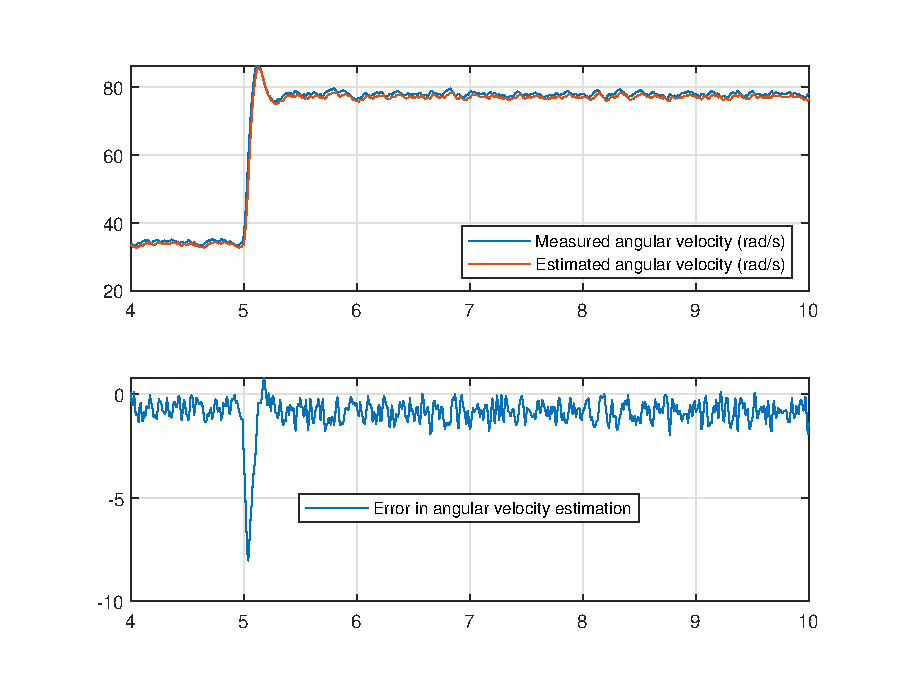
\includegraphics[width=\maxwidth{56.196688409433015em}]{figure_3.eps}
\end{center}


\begin{matlabcode}
figure;
clf;

subplot(2, 1, 1)
title(sprintf('Student ID %s - Current true and estimated state', Students.ID));
% Superpose measured and estimated current
plot(t, i)
hold on
plot(t, xHat(2,:))

legend('Measured current (A)', ...
    'Estimated current (A)', ...
    'location', 'northwest');

xlim([TStart - 1, T])
grid on

subplot(2, 1, 2)
% Plot the error for current here
plot(t, i-xHat(2, :))

legend('Error in current estimation', 'location', 'best');
xlim([TStart - 1, T])
grid on
\end{matlabcode}
\begin{center}
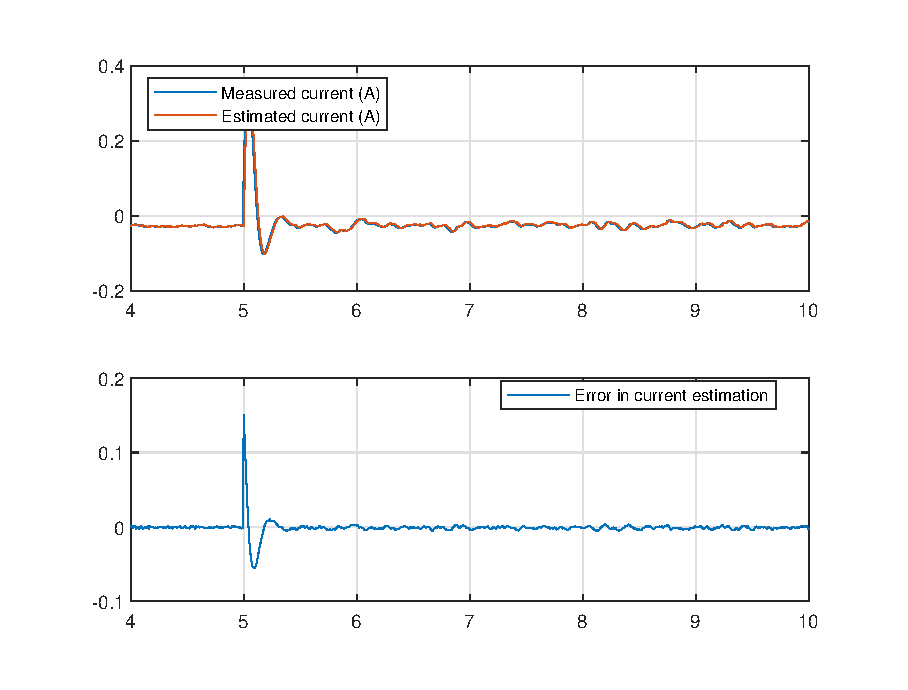
\includegraphics[width=\maxwidth{56.196688409433015em}]{figure_4.eps}
\end{center}

\end{document}
